\section{Additional Checks}
\label{sec:appendix_checks}
This appendix collects the checks that complete the analysis of Secs.~\ref{sec:frequentist}--\ref{sec:validation}. Each one states what it tests and its result, so that it can be read independently.

\subsection{Profile Likelihood, Posterior and the Two Polarities}
\label{sec:checks_profile}
\emph{In short: profiling and marginalizing the nuisance parameters give the same distribution of $A$; the two magnet polarities agree with each other, and combining their likelihoods reproduces the joint fit.}
The frequentist way of eliminating the nuisance parameters is to profile them, $q(A)=-2\Delta\ln L$ with the other parameters re-maximized at each $A$, the Bayesian one is to marginalize them; Fig.~\ref{fig:checks_profile}a shows that $\exp[-q(A)/2]$, normalized, and the marginal posterior coincide, as expected for a near-Gaussian likelihood and flat priors. The two polarities were fitted separately and their profile curves added, which is the combination of likelihoods of two independent measurements of the same parameter (Fig.~\ref{fig:checks_profile}b): magnet down gives $-0.0492\pm0.0111$, magnet up $-0.0374\pm0.0131$, their sum $-0.0443\pm0.0084$, against $-0.0441\pm0.0085$ of the joint fit (the nuisance parameters are shared in the joint fit, separate in the sum). The Bayesian counterpart is sequential: the posterior of magnet down used as the prior of magnet up gives $-0.0446\pm0.0086$ (Table~\ref{tab:checks_polarity}).


\begin{table}[h]
\centering
\resizebox{\ifdim\width>\linewidth\linewidth\else\width\fi}{!}{\begin{tabular}{lcc}
\toprule
 & Frequentist & Bayesian \\
\midrule
Magnet down & $-0.0492\pm0.0111$ & $-0.0497\pm0.0112$ \\
Magnet up & $-0.0374\pm0.0131$ & $-0.0378\pm0.0129$ \\
Combination of the two & $-0.0443\pm0.0084$ & $-0.0446\pm0.0086$ \\
Joint fit & $-0.0441\pm0.0085$ & $-0.0443\pm0.0085$ \\
\bottomrule
\end{tabular}}
\caption{$\Araw$ for the two magnet polarities and their combination, by the two methods; the frequentist combination is the sum of the profile likelihoods of the two polarities, the Bayesian one the sequential update of the posterior.}
\label{tab:checks_polarity}
\end{table}

\subsection{Confidence and Credible Regions in $(A,A_b)$}
\label{sec:checks_region}
\emph{In short: the $68\%$ and $95\%$ regions of the frequentist profile ($\Delta\mathrm{NLL}$ at the $\chi^2_2$ values $2.30$ and $5.99$) and of the Bayesian highest posterior density coincide, and $A=0$ lies outside both.}
For two parameters of interest the Wilks statistic follows a $\chi^2$ with two degrees of freedom (Fig.~\ref{fig:checks_region}). The background asymmetry is $A_b=-0.0402\pm0.0176$ (Hesse; Minos $[-0.0578,-0.0226]$), correlated with $A$ by $\rho=-0.16$ in the likelihood, $-0.17$ in the posterior, and $-0.17$ in the bootstrap. The point $A_b=0$ is at the edge of the $95\%$ region.

\begin{figure}[h]
\centering
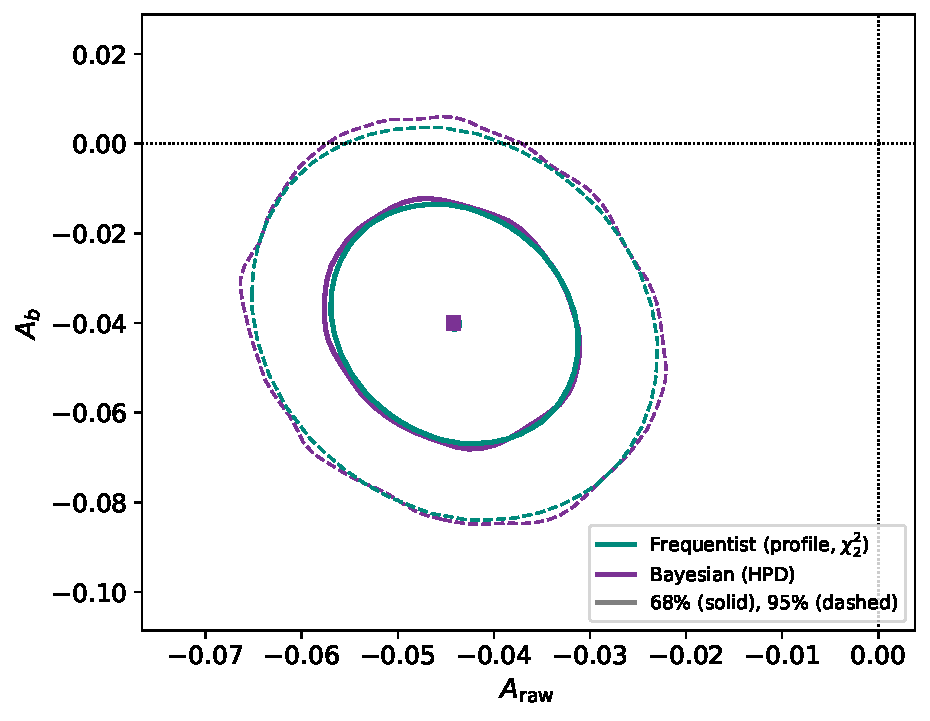
\includegraphics[width=\columnwidth]{figures/validation_region_Ab.pdf}
\caption{$68\%$ (solid) and $95\%$ (dashed) regions in $(A,A_b)$: frequentist, from the profile likelihood with $\chi^2_2$ thresholds, and Bayesian, highest-posterior-density regions of the chain. Dots: best-fit and posterior median.}
\label{fig:checks_region}
\end{figure}

\subsection{Priors and Bayes Factors}
\label{sec:checks_prior}
\emph{In short: no change of the prior on the nuisance parameters or of its parametrization moves $A$ by more than $0.0002$; the Bayes factor of $A=0$ scales with the prior width, and the evidence computed by direct integration agrees in order of magnitude with the Savage-Dickey ratio.}
The posterior was reweighted, without new sampling, to other priors: logarithmically uniform yields and slopes, a prior uniform in the lifetimes $1/\lambda$, and a prior flat in $(N_s^+,N_s^-)$ and $(N_b^+,N_b^-)$ instead of $(N_s,A)$ and $(N_b,A_b)$, which differ by the Jacobian $N_s/2$ (Table~\ref{tab:checks_prior}). The largest shift is $0.0002$, and the effective sample size of the reweighted chain is stated.

\begin{table}[h]
\centering
\resizebox{\ifdim\width>\linewidth\linewidth\else\width\fi}{!}{\begin{tabular}{lccc}
\toprule
Prior & $A$ (median) & $68\%$ interval & ESS \\
\midrule
Nominal (uniform) & $-0.0442$ & $[-0.0529,-0.0358]$ & $20000$ \\
Log-uniform $N_s$, $N_b$ & $-0.0442$ & $[-0.0529,-0.0358]$ & $19993$ \\
Log-uniform slopes & $-0.0440$ & $[-0.0528,-0.0356]$ & $12306$ \\
Uniform in $1/\lambda$ & $-0.0444$ & $[-0.0526,-0.0360]$ & $153$ \\
Flat in $(N_s^+,N_s^-)$ & $-0.0442$ & $[-0.0529,-0.0358]$ & $19999$ \\
Flat in $(N_s^\pm)$ and $(N_b^\pm)$ & $-0.0442$ & $[-0.0529,-0.0358]$ & $19993$ \\
\bottomrule
\end{tabular}}
\caption{Posterior of $A$ under alternative priors, by importance reweighting of the chain; ESS: effective sample size of the $20{,}000$ thinned samples.}
\label{tab:checks_prior}
\end{table}

The Bayes factor $BF_{01}=p(A=0\mid D)/\pi(0)$ is proportional to the density of the prior at zero, $\pi(0)=1/(2W)$ for a uniform prior on $(-W,W)$ (Fig.~\ref{fig:checks_bf}): for $A$ it stays below $10^{-2}$ for every width up to $W=1$ (decisive evidence for $A\neq0$ whatever the prior), while for $A_b$ it crosses $1$ at $W\simeq0.3$, which is the content of the Lindley paradox. The same evidence was computed by direct numerical integration over $A$ on a grid, $Z_1=\int L\,\pi\,dA$ with the nuisance parameters fixed at the maximum of the posterior, the method that is not feasible for twelve parameters: it gives $K_{01}=7.0e-05$, against $1.3e-04$ with the profile likelihood and $1.1e-04$ for the Savage-Dickey ratio, which marginalizes the nuisance parameters; the three values are of the same order and the conclusion is the same.


The Savage-Dickey ratio also tests the equality of the background shapes of the two charges, one parameter at a time, with the difference $\delta=\theta^+-\theta^-$: $BF_{01}=3.1$ for the steep slope $\lambda_1$ (difference at $0.8\sigma$), $2.2$ for $\lambda_2$ ($2.4\sigma$) and $1.1$ for the fraction $f$ ($2.0\sigma$). The data are not able to distinguish the shapes, with a weak preference for equal ones: this is why the variant with a shared shape moves $A$ by $-0.0037$ and is part of the systematic uncertainty, without being preferred.

\subsection{Equal-Tailed and Highest-Posterior-Density Intervals}
\label{sec:checks_hpd}
\emph{In short: for $A$ and $A_b$ the two kinds of $68\%$ interval coincide; they differ for the skewed parameters, whose highest-posterior-density interval is shifted towards the mode.}
Table~\ref{tab:checks_hpd} compares the equal-tailed interval (percentiles $15.9\%$--$84.1\%$) with the interval of highest posterior density, the shortest containing $68.3\%$, for the parameters of interest and for three skewed nuisance parameters.

\begin{table}[h]
\centering
\resizebox{\ifdim\width>\linewidth\linewidth\else\width\fi}{!}{\begin{tabular}{lcccc}
\toprule
Parameter & median & equal-tailed & HPD & skewness \\
\midrule
$A$ & $-0.0442$ & $[-0.0529,-0.0358]$ & $[-0.0525,-0.0355]$ & $+0.01$ \\
$A_b$ & $-0.0400$ & $[-0.0575,-0.0224]$ & $[-0.0575,-0.0225]$ & $+0.01$ \\
$f_+$ & $0.114$ & $[0.089,0.145]$ & $[0.084,0.138]$ & $+0.90$ \\
$f_-$ & $0.209$ & $[0.174,0.248]$ & $[0.168,0.241]$ & $+0.33$ \\
$\lambda_1^+$ [MeV$^{-1}$] & $0.0350$ & $[0.0281,0.0431]$ & $[0.0274,0.0423]$ & $+0.52$ \\
\bottomrule
\end{tabular}}
\caption{Equal-tailed and highest-posterior-density $68\%$ intervals and skewness of the marginal posteriors.}
\label{tab:checks_hpd}
\end{table}

\subsection{Posterior Predictive Check with Statistics Not Fitted by the Model}
\label{sec:checks_ppc}
\emph{In short: the asymmetry in slices of the mass, which the model predicts, is reproduced ($p_B=0.67$), and the difference between the $\chi^2$ of the two charges is at the edge of the replicas ($p_B=0.08$).}
Section~\ref{sec:bayes_gof} noted that the counting asymmetries of the window are fitted by construction. Two statistics that are not adjusted directly were therefore used (Fig.~\ref{fig:checks_ppc}): the asymmetry in ten slices of $50\,\MeV$ of the mass against the one predicted by the model from the same posterior draw, which tests that the charge asymmetry follows the mixture of signal and background, $T=\sum_s(A_s-\bar A_s)^2/\sigma_s^2$, and the difference $\chi^2(B^+)-\chi^2(B^-)$ of the binned fit. The slice asymmetries are reproduced; the difference of the $\chi^2$ is $27$ in the data against $-0\pm15$ in the replicas, a $1.8\sigma$ excess that restates that the misfit is concentrated in the $B^+$ sample.

\begin{figure*}[t]
\centering
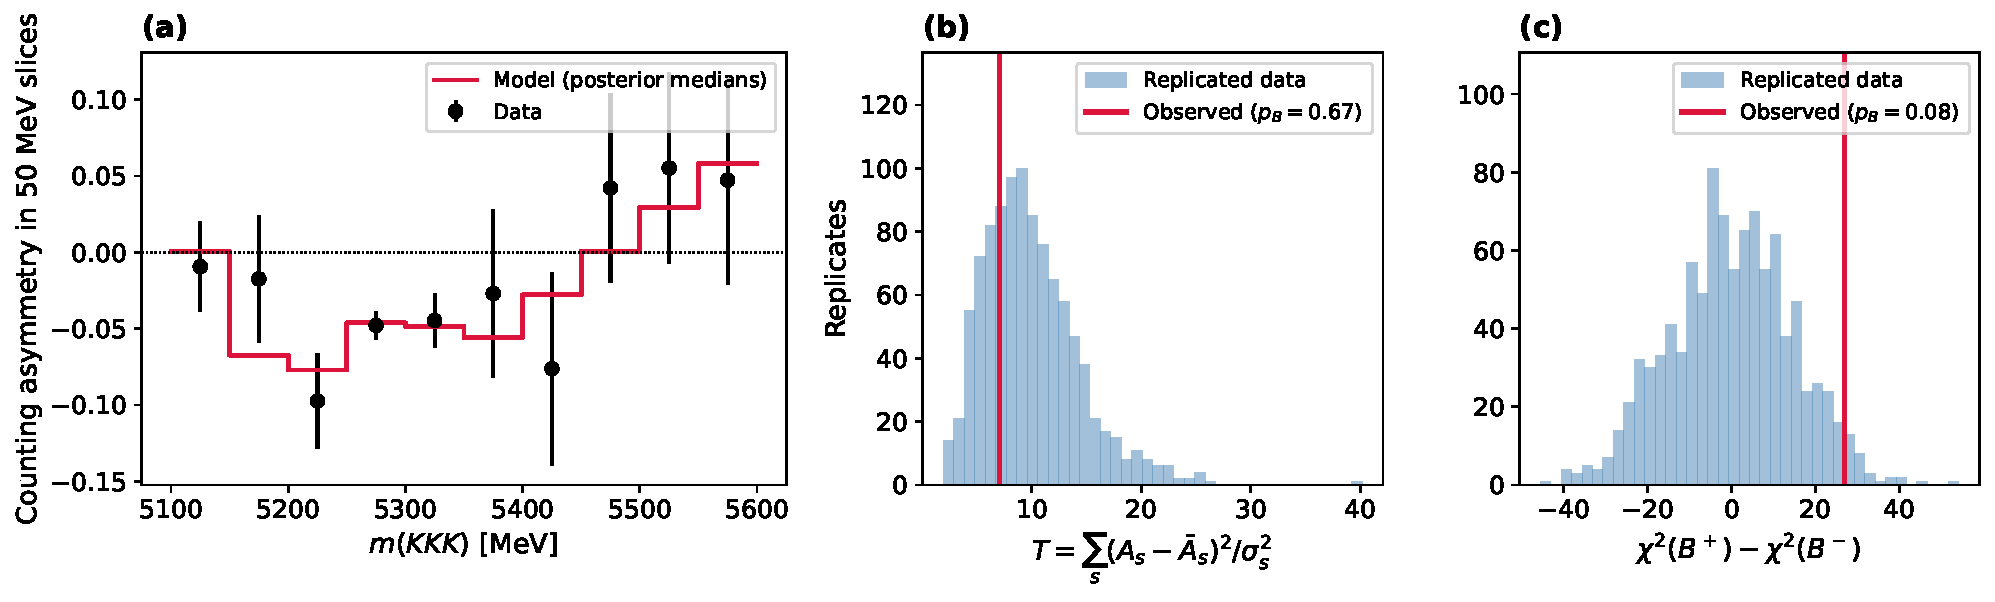
\includegraphics[width=0.95\textwidth]{figures/validation_ppc_unfitted.pdf}
\caption{(a) Counting asymmetry in slices of $50\,\MeV$ of the mass, data and model. (b) Distribution of $T=\sum_s(A_s-\bar A_s)^2/\sigma_s^2$ over $1000$ replicas and observed value. (c) The same for $\chi^2(B^+)-\chi^2(B^-)$.}
\label{fig:checks_ppc}
\end{figure*}

\subsection{Asymptotic Behavior of the Estimator}
\label{sec:checks_scaling}
\emph{In short: with the number of candidates the bias tends to zero, the spread scales as $N^{-1/2}$ and the distribution of $\hat A$ becomes Gaussian, as the central limit theorem and the asymptotic properties of the maximum-likelihood estimate predict.}
The $300$ toy-MC datasets for each size of the low-statistics study (Sec.~\ref{sec:bayes_lowstat}) show the approach to the asymptotic limit (Table~\ref{tab:checks_scaling}): the bias decreases from $-0.0085$ at $N=50$ to $+0.0009$ at $N=2000$, the product of the spread and $\sqrt N$ is constant, and the distribution of $\hat A$ is compatible with a Gaussian from $N=150$ (Shapiro-Wilk $p>0.3$), with a mild excess kurtosis at $N=50$ ($p=0.03$). Linear propagation of the Poisson uncertainty of the signal yield, $\sigma(A)=\sqrt{(1-A^2)/N_s}$ with $N_s=0.86\,N$, gives $0.153$ at $N=50$ and $0.024$ at $N=2000$, against spreads of $0.161$ and $0.023$: it is correct at the few-per-cent level, because the fit also has to determine the background, and the first-order expansion is not the limiting approximation. At the full sample the spread of the estimator equals the Hesse uncertainty (Sec.~\ref{sec:validation_estimator}).

\begin{table}[h]
\centering
\resizebox{\ifdim\width>\linewidth\linewidth\else\width\fi}{!}{\begin{tabular}{rcccccc}
\toprule
$N$ & bias & sd$(\hat A)$ & sd$\cdot\sqrt N$ & skewness & ex.\ kurtosis & Shapiro $p$ \\
\midrule
$50$ & $-0.0085$ & $0.1611$ & $1.14$ & $-0.15$ & $+0.64$ & $0.03$ \\
$150$ & $-0.0051$ & $0.0920$ & $1.13$ & $+0.16$ & $+0.31$ & $0.59$ \\
$500$ & $-0.0022$ & $0.0501$ & $1.12$ & $-0.08$ & $+0.38$ & $0.52$ \\
$2000$ & $+0.0009$ & $0.0225$ & $1.01$ & $-0.20$ & $-0.20$ & $0.32$ \\
\bottomrule
\end{tabular}}
\caption{Distribution of the maximum-likelihood estimate of $A$ in $300$ toy-MC datasets of $N$ candidates (six-parameter model of Sec.~\ref{sec:bayes_minimal}).}
\label{tab:checks_scaling}
\end{table}

\subsection{Uncertainties of the Twelve Parameters by Three Methods}
\label{sec:checks_covariance}
\emph{In short: the inverse of the Fisher information (Hesse), the bootstrap of the data and the posterior give the same standard deviations, except for the two yields in the bootstrap, which keeps the total number of candidates fixed.}
The covariance of the fit parameters was estimated in three ways (Table~\ref{tab:checks_covariance}): the inverse of the matrix of second derivatives of $-\ln L$ at the minimum (Hesse), $300$ bootstrap replicas of the data, each refitted, and the posterior sample. They agree to $10\%$ for all the shape parameters and for $A$, $A_b$, $\mu$ and $\sigma$. The exception is the signal and background yields, $\sigma(N_s)=133$ (Hesse) and $72$ (bootstrap): a resampling of $N$ candidates keeps the total yield fixed, which the extended likelihood does not, and the yields of the bootstrap show the anticorrelated fluctuation of the binomial split; the asymmetry $A$ is not affected. The correlation between $A$ and $A_b$ is $-0.16$, $-0.17$ and $-0.17$ in the three methods.

\begin{table}[h]
\centering
\begin{tabular}{lccc}
\toprule
Parameter & Hesse & Bootstrap & Posterior \\
\midrule
$A$ & $0.0085$ & $0.0085$ & $0.0085$ \\
$A_b$ & $0.0177$ & $0.0183$ & $0.0176$ \\
$N_s$ & $133$ & $72$ & $133$ \\
$N_b$ & $82$ & $72$ & $82$ \\
$\mu$ [MeV] & $0.159$ & $0.159$ & $0.161$ \\
$\sigma$ [MeV] & $0.141$ & $0.150$ & $0.138$ \\
$\lambda_1^+$ & $0.0077$ & $0.0057$ & $0.0078$ \\
$\lambda_2^+$ & $0.00028$ & $0.00030$ & $0.00029$ \\
$f_+$ & $0.028$ & $0.029$ & $0.030$ \\
$\lambda_1^-$ & $0.0047$ & $0.0043$ & $0.0047$ \\
$\lambda_2^-$ & $0.00040$ & $0.00038$ & $0.00039$ \\
$f_-$ & $0.039$ & $0.036$ & $0.037$ \\
\bottomrule
\end{tabular}
\caption{Standard deviation of the parameters of the nominal fit from the Hesse matrix, from the bootstrap of the data and from the posterior.}
\label{tab:checks_covariance}
\end{table}

\subsection{Starting Values and Weakly Constrained Parameters}
\label{sec:checks_multistart}
\emph{In short: $29$ of $30$ fits from random starting points reach the same minimum; the steep-background fraction is the weakly constrained direction, as the long chain of the Bayesian fit already showed.}
The nominal fit was repeated from $30$ starting points drawn at random (yields and slopes multiplied by a log-normal factor of width $0.5$, the fractions uniform, the asymmetry uniform in $(-0.2,0.2)$): $29$ reach the minimum of the nominal fit ($\hat A=-0.0441$); the remaining one stops in a local minimum $96$ units of $-2\ln L$ above, at $\hat A=-0.052$, which would be rejected by comparing the likelihood values. The profile likelihood of the fraction of the steep component for $B^+$ (the parameter whose chain mixes slowly in the narrow window, Sec.~\ref{sec:bayes_gof}) is asymmetric: $q(f_+)=1$ at $0.085$ and $0.140$ around the best value $0.112$, with a longer tail towards large fractions where the two exponentials exchange their roles. The uncertainty of $A$ does not depend on it (correlation below $0.1$).

\subsection{Validation of the Rule for Nested Samples}
\label{sec:checks_barlow}
\emph{In short: the spread of the shift of $\hat A$ between a sample and its tighter-identification subsample is the one given by the quadrature difference of the uncertainties.}
The systematic study counts a variant that changes the sample only if its shift exceeds $\sigma_B=\sqrt{|\sigma_{\mathrm{var}}^2-\sigma_{\mathrm{nom}}^2|}$ (Sec.~\ref{sec:syst}). To verify the rule, $300$ bootstrap replicas of the nominal sample were fitted before and after the tighter selections $\texttt{ProbK}>0.6$ and $\texttt{ProbPi}<0.4$ (Fig.~\ref{fig:checks_barlow}): the standard deviation of the shift is $0.0051$ and $0.0025$, against median $\sigma_B$ of $0.0050$ and $0.0023$ (ratios $1.02$ and $1.09$), and the shifts follow a Gaussian of width $\sigma_B$. The mean shift of the replicas ($0.0060$ and $0.0020$) is that of the data, which is preserved by the resampling: it is a property of the sample and not a fluctuation of the rule.

\begin{figure*}[t]
\centering
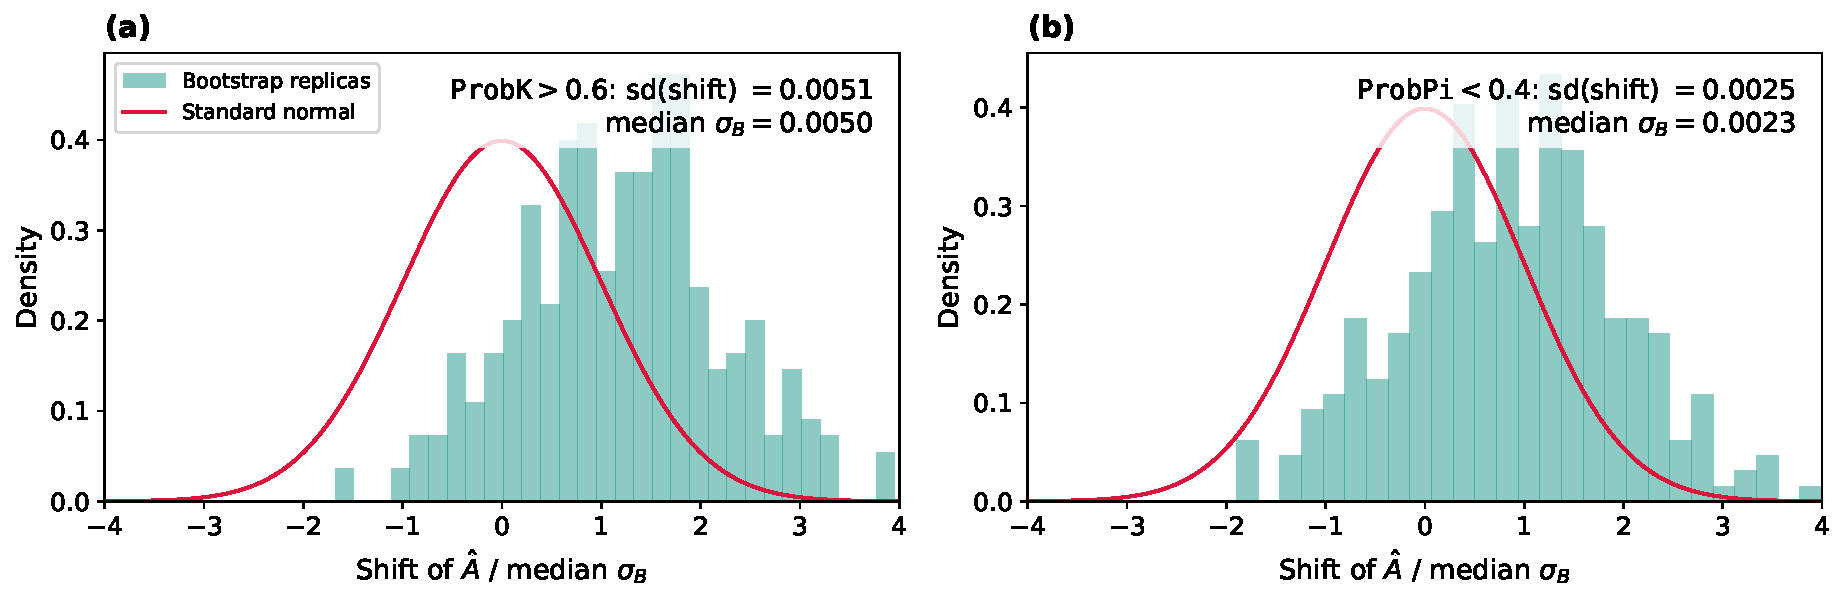
\includegraphics[width=0.95\textwidth]{figures/validation_barlow.pdf}
\caption{Shift of $\hat A$ between the nominal sample and a tighter selection, divided by the median $\sigma_B$, in $300$ bootstrap replicas of the data: (a) $\texttt{ProbK}>0.6$, (b) $\texttt{ProbPi}<0.4$, and standard normal distribution.}
\label{fig:checks_barlow}
\end{figure*}

\subsection{Neyman Construction and Dependence on the Momentum}
\label{sec:checks_belt}
\emph{In short: inverting the test of $A_{\mathrm{true}}$ with toy-MC experiments gives the same interval as the likelihood ratio, and $\Araw$ does not depend on the momentum of the $B$.}
The confidence interval is, by definition, the set of $A_{\mathrm{true}}$ not rejected by the data. It was constructed directly (Fig.~\ref{fig:checks_belt}): for $11$ values of $A_{\mathrm{true}}$ between $-0.1$ and $0$, $300$ toy-MC experiments give the central $68\%$ and $95\%$ ranges of $\hat A$ (the belt), and the interval is the set of $A_{\mathrm{true}}$ whose $68\%$ range contains the observed $\hat A=-0.0441$: $[-0.0528,-0.0351]$, against $[-0.0526,-0.0356]$ from the profile likelihood (Minos), which is the content of Wilks' theorem for this problem.

\begin{figure}[h]
\centering
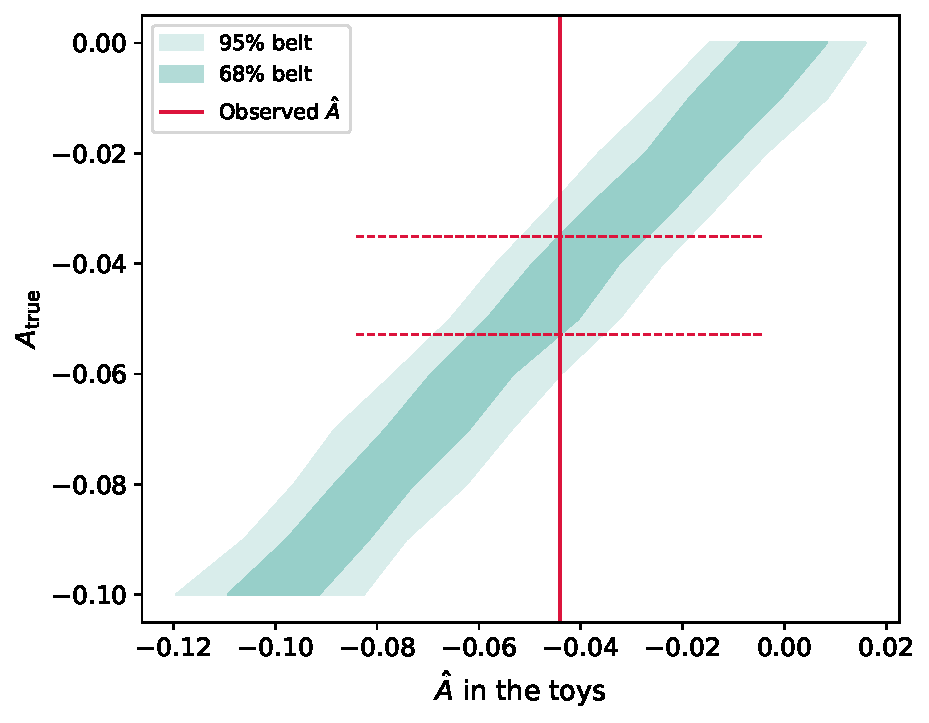
\includegraphics[width=\columnwidth]{figures/validation_neyman_belt.pdf}
\caption{Confidence belt of $\hat A$ from toy-MC experiments (central $68\%$ and $95\%$ ranges) as a function of $A_{\mathrm{true}}$; the vertical line is the observed $\hat A$ and the dashed lines the resulting $68\%$ interval.}
\label{fig:checks_belt}
\end{figure}

The detection asymmetry of kaons depends on their momentum; as a direct check, the joint fit was repeated in three bins with equal numbers of candidates of the transverse momentum $p_T$ and of the momentum $p$ of the $B$ candidate (Table~\ref{tab:checks_momentum}): the three values are compatible with the global one, with a largest deviation of $1.4\sigma$.

\begin{table}[h]
\centering
\begin{tabular}{lccc}
\toprule
Bin & range [GeV] & $n$ & $\Araw$ \\
\midrule
$p_T$, 1 & $1.0$--$4.7$ & $6577$ & $-0.0563\pm0.0169$ \\
$p_T$, 2 & $4.7$--$8.2$ & $6577$ & $-0.0362\pm0.0141$ \\
$p_T$, 3 & $8.2$--$30.5$ & $6577$ & $-0.0452\pm0.0134$ \\
$p$, 1 & $26.7$--$78.1$ & $6577$ & $-0.0391\pm0.0139$ \\
$p$, 2 & $78.1$--$110.1$ & $6577$ & $-0.0475\pm0.0149$ \\
$p$, 3 & $110.1$--$288.5$ & $6577$ & $-0.0478\pm0.0153$ \\
\bottomrule
\end{tabular}
\caption{$\Araw$ (joint frequentist fit) in terciles of the transverse momentum and of the momentum of the $B$ candidate.}
\label{tab:checks_momentum}
\end{table}

\subsection{Metropolis-Hastings Sampler and Published Likelihood}
\label{sec:checks_mh}
\emph{In short: an own Metropolis-Hastings sampler reproduces the posterior of the ensemble sampler, and the profile likelihood is given in a table, so that the result can be combined with others.}
The algorithm of the ensemble sampler was replaced by the basic Metropolis-Hastings one: a Gaussian proposal with the covariance of the posterior scaled by $2.38^2/d$, $120{,}000$ steps with the first $1/6$ discarded. The acceptance is $0.24$, the integrated autocorrelation time of $A$ is $36$ steps ($2813$ effective samples), and $A=-0.0443$ with $68\%$ interval $[-0.0526,-0.0357]$, against $-0.0443$ and $[-0.0528,-0.0358]$ from the ensemble sampler: the two samplers give the same posterior.

The profile likelihood of $A$ is given in Table~\ref{tab:checks_qa}, together with the Minos intervals, so that other measurements of the same quantity can be combined with this one by adding $q(A)$.

\begin{table}[h]
\centering
\resizebox{\ifdim\width>\linewidth\linewidth\else\width\fi}{!}{\begin{tabular}{r|ccccccccc}
\toprule
$A$ & $-0.08$ & $-0.07$ & $-0.06$ & $-0.05$ & $-0.04$ & $-0.03$ & $-0.02$ & $-0.01$ & $+0.00$ \\
$q(A)$ & $17.9$ & $9.3$ & $3.5$ & $0.5$ & $0.2$ & $2.8$ & $8.1$ & $16.1$ & $27.0$ \\
\bottomrule
\end{tabular}}
\caption{Profile likelihood ratio $q(A)=-2\Delta\ln L$ of the nominal fit (other parameters profiled); minimum at $-0.0441$, Minos intervals $[-0.0526,-0.0356]$ ($68\%$) and $[-0.0607,-0.0275]$ ($95\%$).}
\label{tab:checks_qa}
\end{table}
